\chapter{SGANs approximate Jensen–Shannon Divergence}

\label{apx:JSD}

% If there are several additions you want to add, but they do not fit into the thesis itself, they belong here.

% \section{Detailed Addition}

% Even sections are possible, but usually only used for several elements in, e.g.\ tables, images, etc.
\let\oldclearpage\clearpage
\let\clearpage\relax
\chapter{Circuits}
\section{SQGANs Ansatz}
\label{apx:sqgans_ansatz}


\section{Topological Phase Transition Ansatz}
\label{apx:topological_phase_transition_ansatz}

\section{Butterfly Ansatz}
\label{apx:butterfly_ansatz}

\chapter{SQGANs Cost Function}
\label{apx:sqgans_cost_function}

\chapter{Optimizer Setup}
\label{apx:optimizer_setup}
Short description of Adam and meta parameters used (they change in different
setting, so it must be mentioned in the main text)

\chapter{Additional Results}
\section{WQGANs Results}
\label{apx:wqgans_pahse_results}
\begin{figure}[htbp!]
  \captionsetup[subfigure]{labelformat=empty}
  \centering
  \subfloat{
    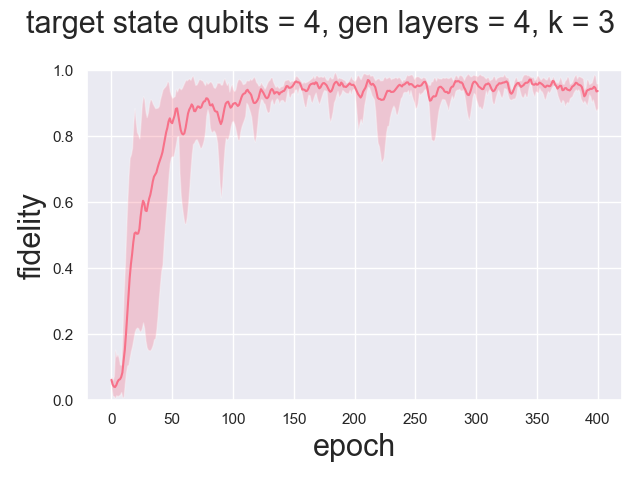
\includegraphics[width=0.3\linewidth]{figures/wqgans_phase_size=4_k=3_gen=4/fidelity.png}
  }
  \subfloat{
    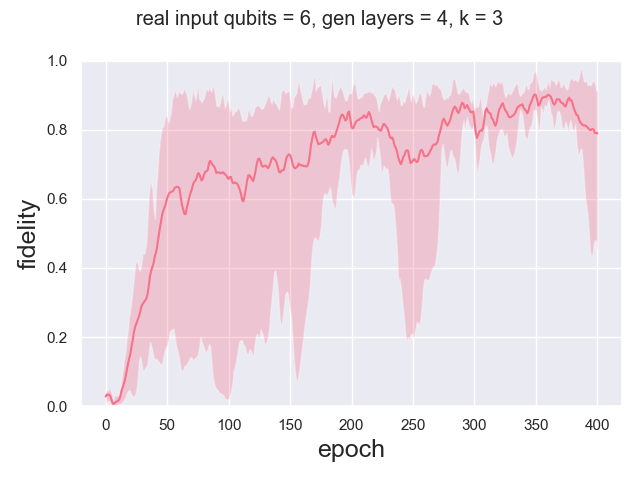
\includegraphics[width=0.3\linewidth]{figures/wqgans_phase_size=6_k=3_gen=4/fidelity.png}
  }
  \subfloat{
    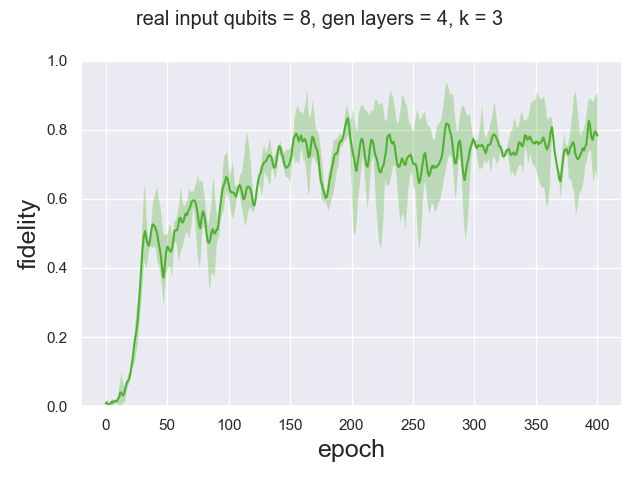
\includegraphics[width=0.3\linewidth]{figures/wqgans_phase_size=8_k=3_gen=4/fidelity.png}
  }

  \subfloat{
    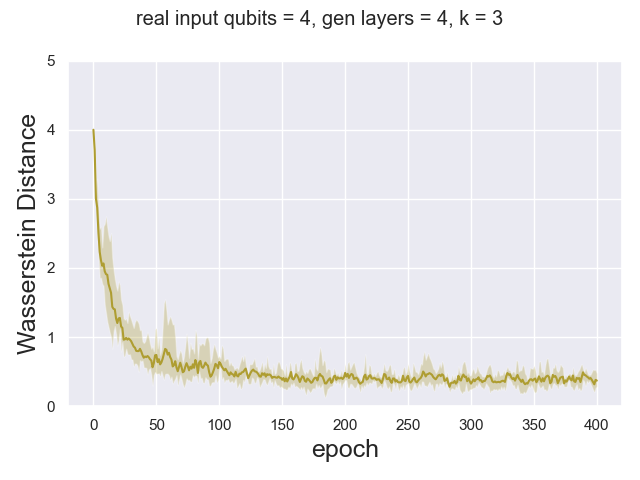
\includegraphics[width=0.3\linewidth]{figures/wqgans_phase_size=4_k=3_gen=4/Wasserstein_Distance.png}
  }
  \subfloat{
    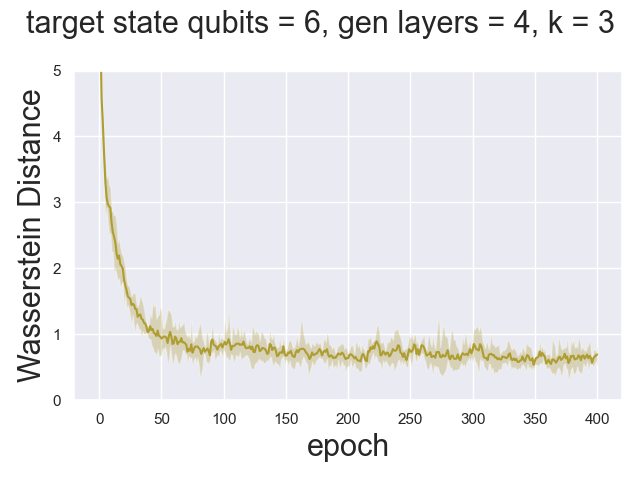
\includegraphics[width=0.3\linewidth]{figures/wqgans_phase_size=6_k=3_gen=4/Wasserstein_Distance.png}
  }
  \subfloat{
    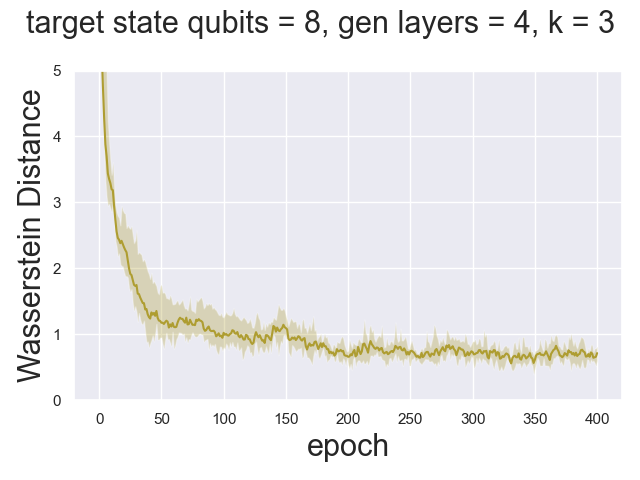
\includegraphics[width=0.3\linewidth]{figures/wqgans_phase_size=8_k=3_gen=4/Wasserstein_Distance.png}
  }
  \caption{The solid line represents the average value and the shaded area
    represents the range from 5 different experiments. }
  \label{fig:wqgans_phase_res_2}
\end{figure}


\begin{figure}[htbp!]
  \captionsetup[subfigure]{labelformat=empty}
  \centering
  \subfloat{
    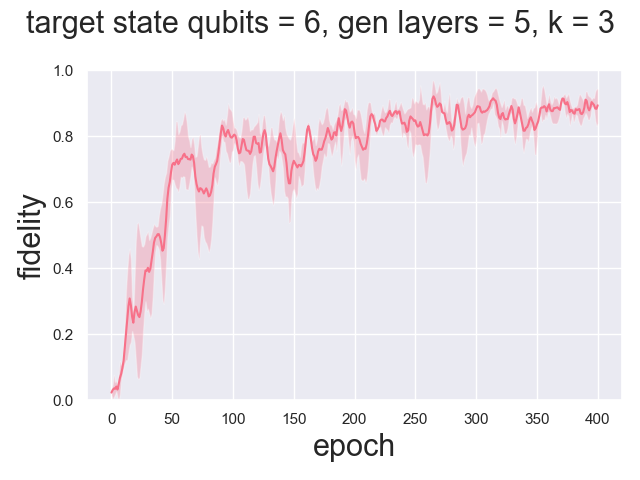
\includegraphics[width=0.3\linewidth]{figures/wqgans_phase_size=6_k=3_gen=5/fidelity.png}
  }
  \subfloat{
    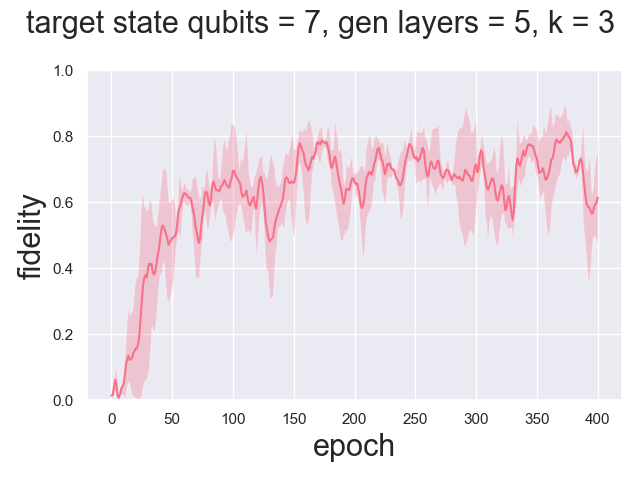
\includegraphics[width=0.3\linewidth]{figures/wqgans_phase_size=7_k=3_gen=5/fidelity.png}
  }
  \subfloat{
    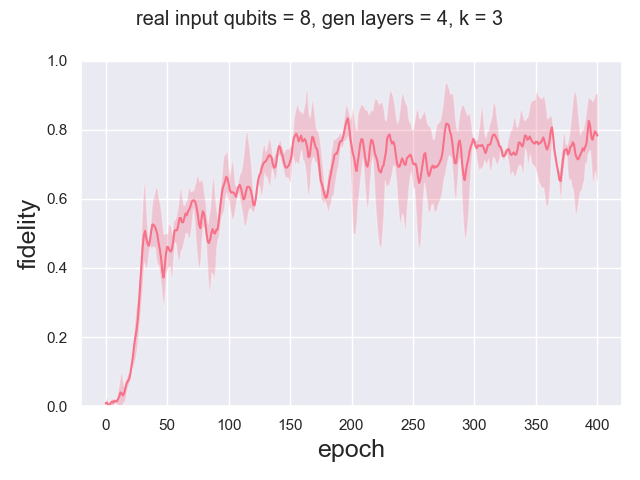
\includegraphics[width=0.3\linewidth]{figures/wqgans_phase_size=8_k=3_gen=5/fidelity.png}
  }

  \subfloat{
    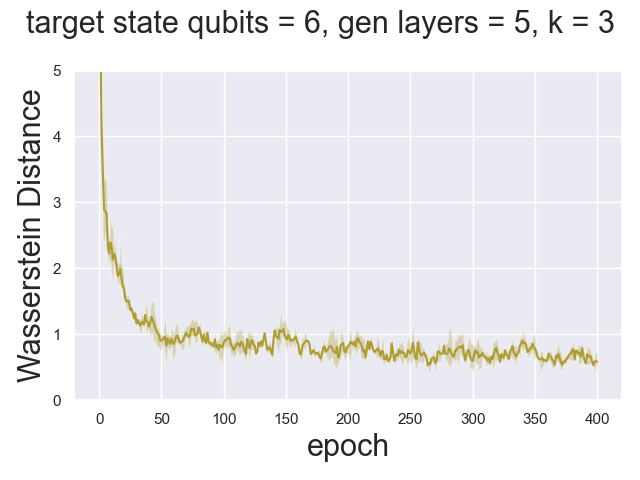
\includegraphics[width=0.3\linewidth]{figures/wqgans_phase_size=6_k=3_gen=5/Wasserstein_Distance.png}
  }
  \subfloat{
    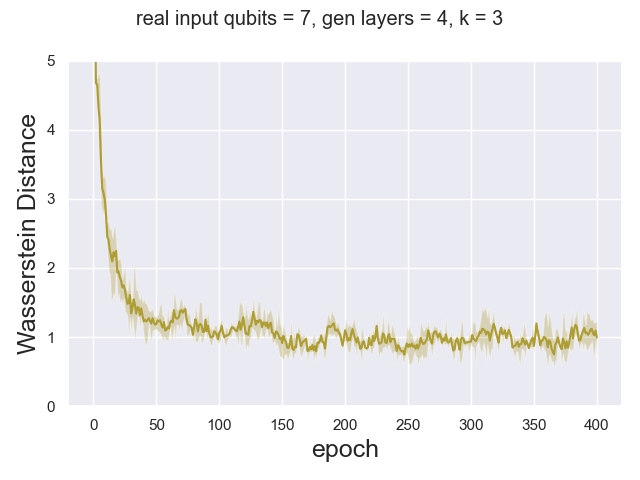
\includegraphics[width=0.3\linewidth]{figures/wqgans_phase_size=7_k=3_gen=5/Wasserstein_Distance.png}
  }
  \subfloat{
    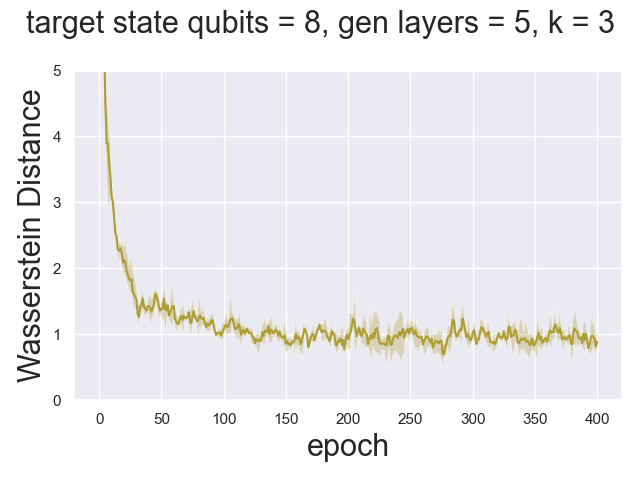
\includegraphics[width=0.3\linewidth]{figures/wqgans_phase_size=8_k=3_gen=5/Wasserstein_Distance.png}
  }
  \caption{The solid line represents the average value and the shaded area
    represents the range from 5 different experiments. }
  \label{fig:wqgans_phase_res_3}
\end{figure}


\begin{figure}[htbp!]
  \captionsetup[subfigure]{labelformat=empty}
  \centering
  \subfloat{
    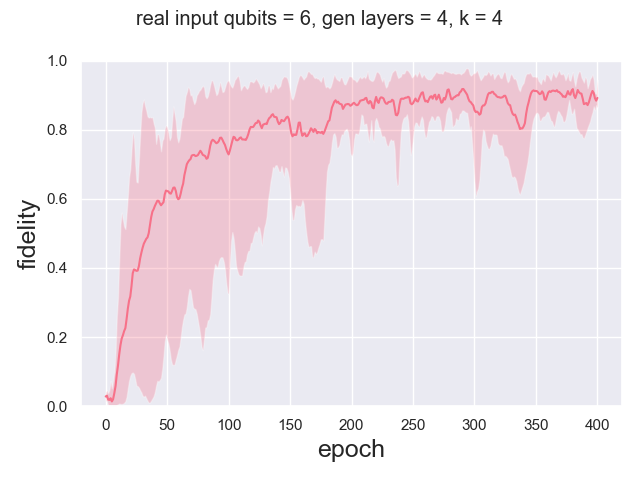
\includegraphics[width=0.3\linewidth]{figures/wqgans_phase_size=6_k=4_gen=4/fidelity.png}
  }
  \subfloat{
    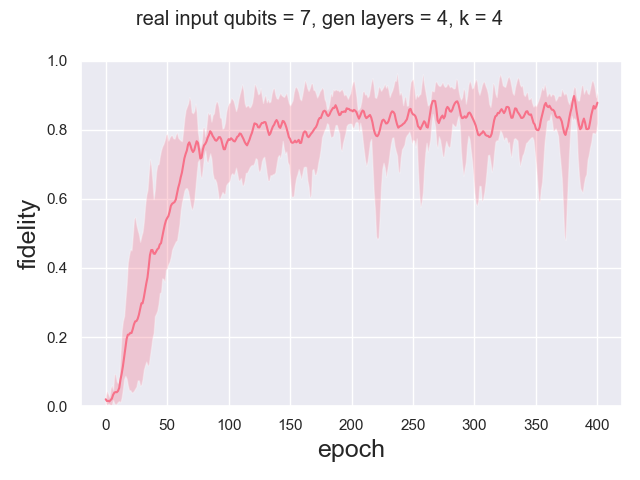
\includegraphics[width=0.3\linewidth]{figures/wqgans_phase_size=7_k=4_gen=4/fidelity.png}
  }
  \subfloat{
    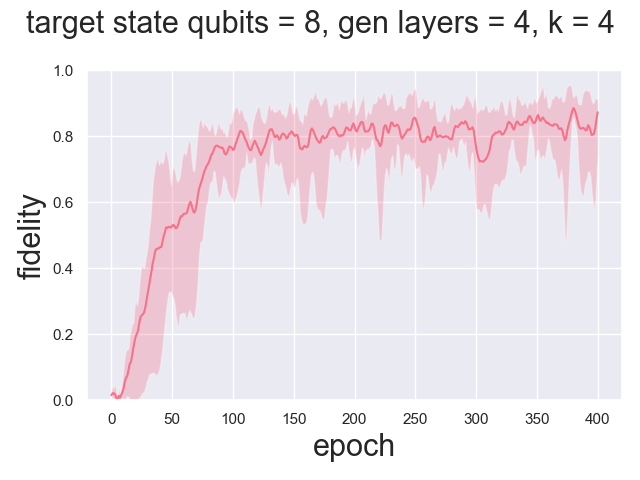
\includegraphics[width=0.3\linewidth]{figures/wqgans_phase_size=8_k=4_gen=4/fidelity.png}
  }

  \subfloat{
    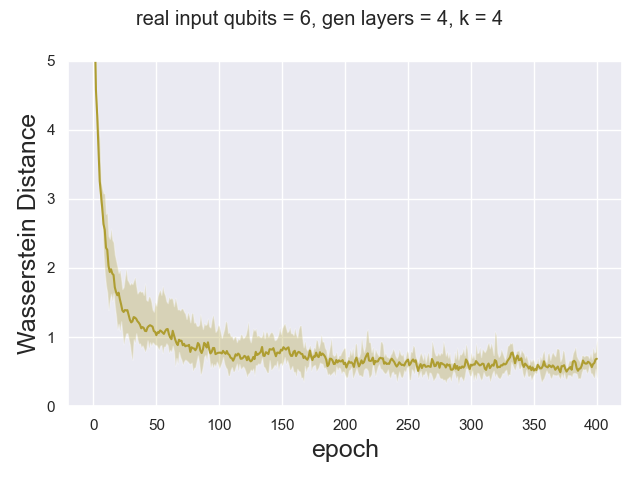
\includegraphics[width=0.3\linewidth]{figures/wqgans_phase_size=6_k=4_gen=4/Wasserstein_Distance.png}
  }
  \subfloat{
    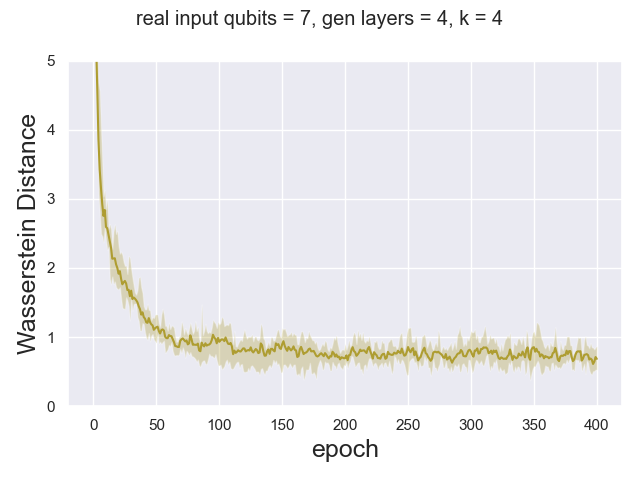
\includegraphics[width=0.3\linewidth]{figures/wqgans_phase_size=7_k=4_gen=4/Wasserstein_Distance.png}
  }
  \subfloat{
    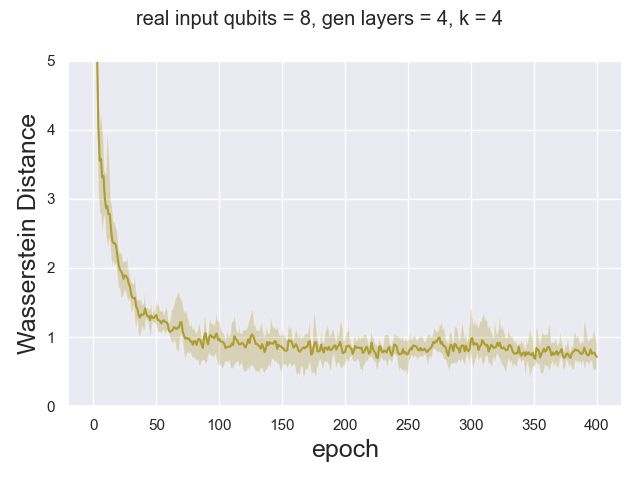
\includegraphics[width=0.3\linewidth]{figures/wqgans_phase_size=8_k=4_gen=4/Wasserstein_Distance.png}
  }
  \caption{The solid line represents the average value and the shaded area
    represents the range from 5 different experiments. }
  \label{fig:wqgans_phase_res_4}
\end{figure}


\begin{figure}[htbp!]
  \captionsetup[subfigure]{labelformat=empty}
  \centering
  \subfloat{
    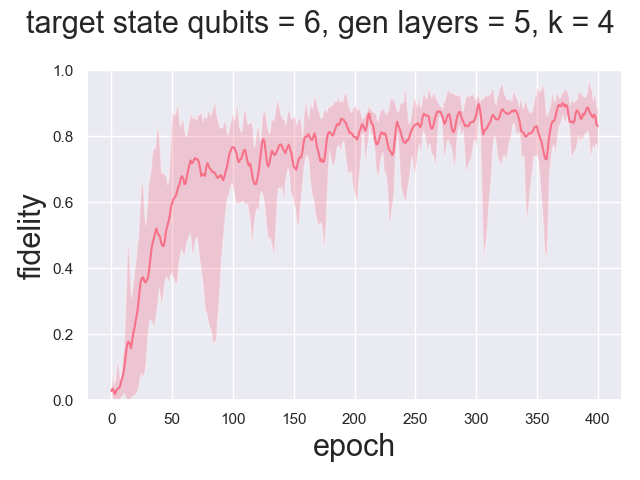
\includegraphics[width=0.3\linewidth]{figures/wqgans_phase_size=6_k=4_gen=5/fidelity.png}
  }
  \subfloat{
    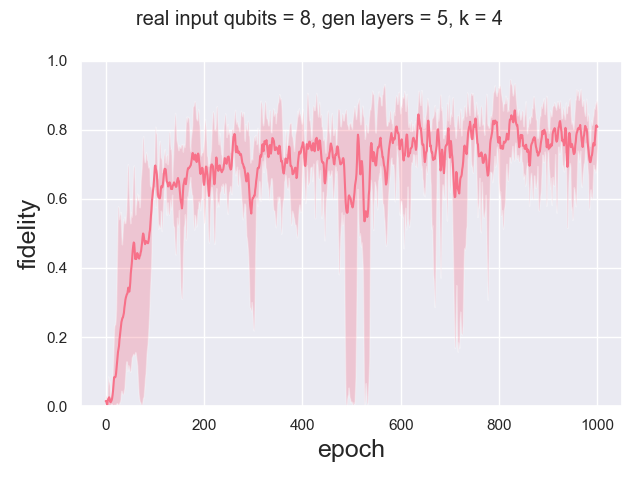
\includegraphics[width=0.3\linewidth]{figures/wqgans_phase_size=8_k=4_gen=5/fidelity.png}
  }
  \subfloat{
    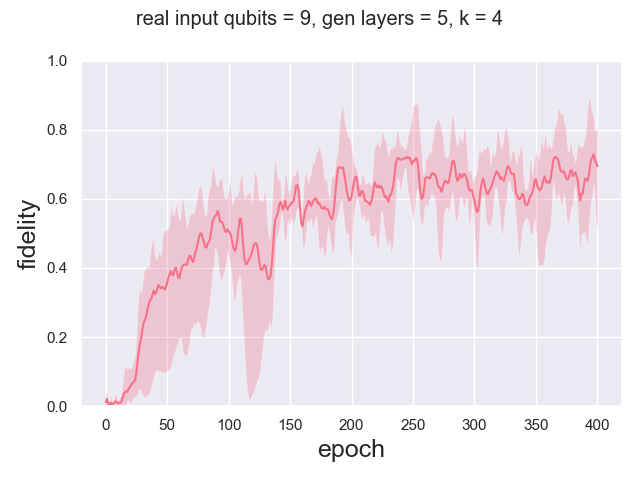
\includegraphics[width=0.3\linewidth]{figures/wqgans_phase_size=9_k=4_gen=5/fidelity.png}
  }

  \subfloat{
    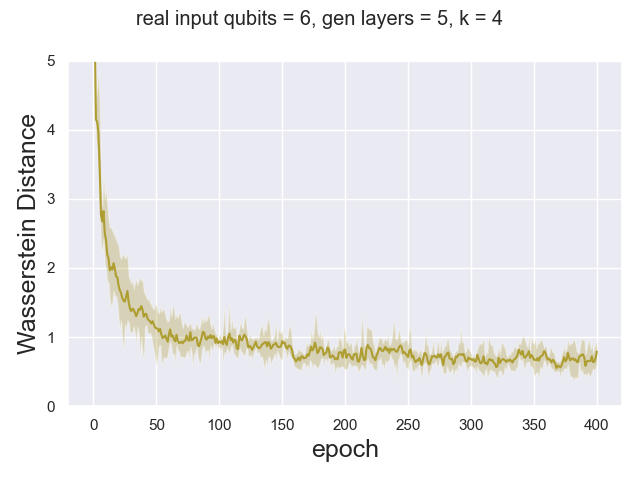
\includegraphics[width=0.3\linewidth]{figures/wqgans_phase_size=6_k=4_gen=5/Wasserstein_Distance.png}
  }
  \subfloat{
    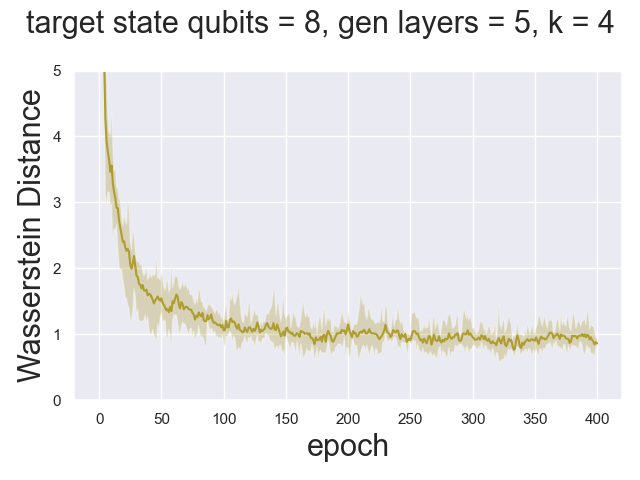
\includegraphics[width=0.3\linewidth]{figures/wqgans_phase_size=8_k=4_gen=5/Wasserstein_Distance.png}
  }
  \subfloat{
    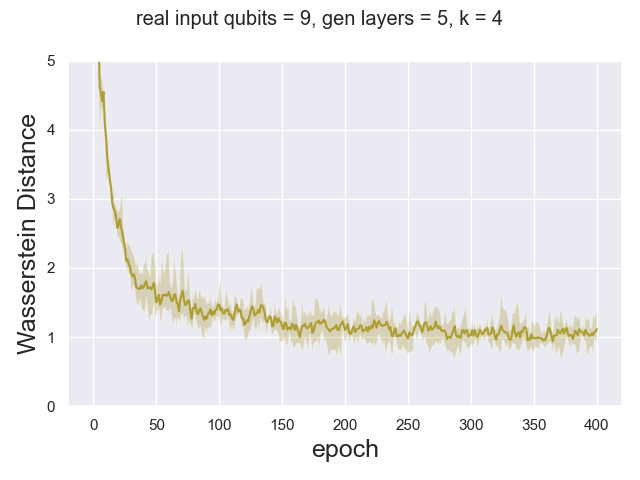
\includegraphics[width=0.3\linewidth]{figures/wqgans_phase_size=9_k=4_gen=5/Wasserstein_Distance.png}
  }
  \caption{The solid line represents the average value and the shaded area
    represents the range from 5 different experiments. }
  \label{fig:wqgans_phase_res_5}
\end{figure}
\label{apx:wqgans_pahse_results_butterfly}

\begin{figure}[htbp!]
  \captionsetup[subfigure]{labelformat=empty}
  \centering
  \subfloat{
    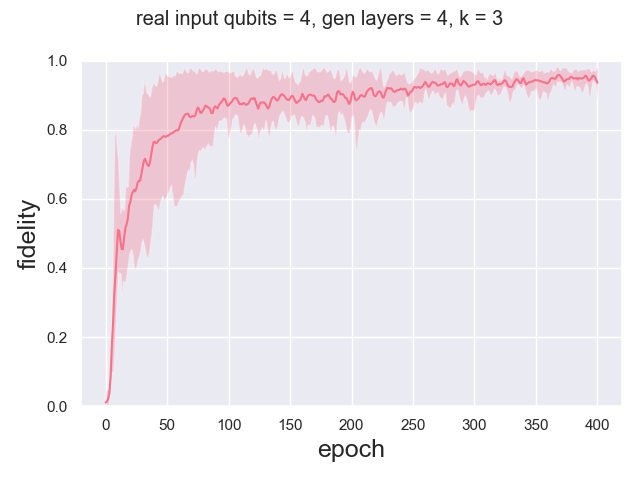
\includegraphics[width=0.25\linewidth]{figures/wqgans_butterfly_size=4_k=3_gen=4/fidelity.png}
  }
  \subfloat{
    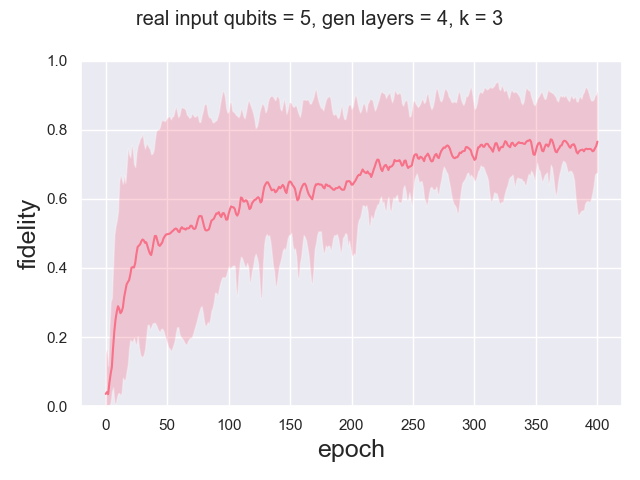
\includegraphics[width=0.25\linewidth]{figures/wqgans_butterfly_size=5_k=3_gen=4/fidelity.png}
  }
  \subfloat{
    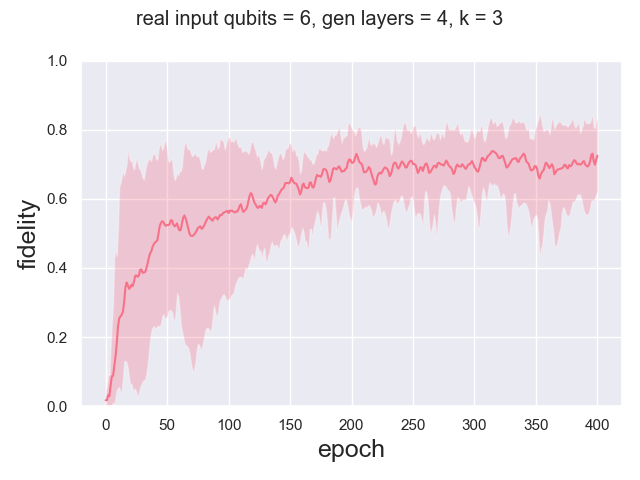
\includegraphics[width=0.25\linewidth]{figures/wqgans_butterfly_size=6_k=3_gen=4/fidelity.png}
  }
  \subfloat{
    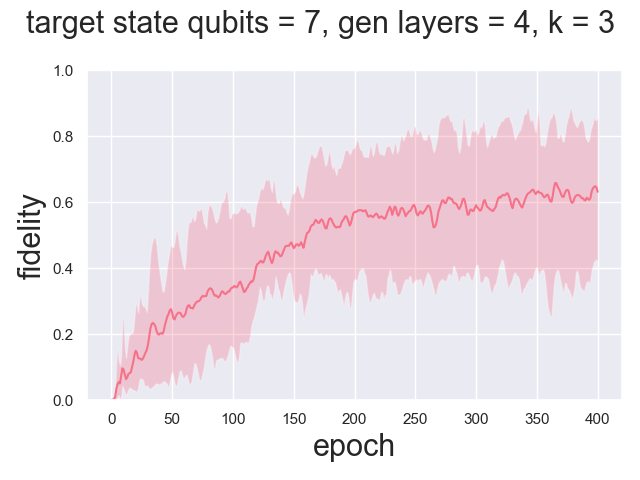
\includegraphics[width=0.25\linewidth]{figures/wqgans_butterfly_size=7_k=3_gen=4/fidelity.png}
  }

  \subfloat{
    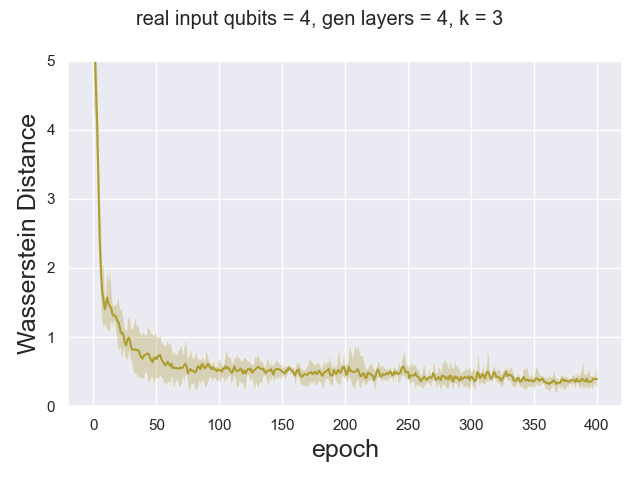
\includegraphics[width=0.25\linewidth]{figures/wqgans_butterfly_size=4_k=3_gen=4/Wasserstein_Distance.png}
  }
  \subfloat{
    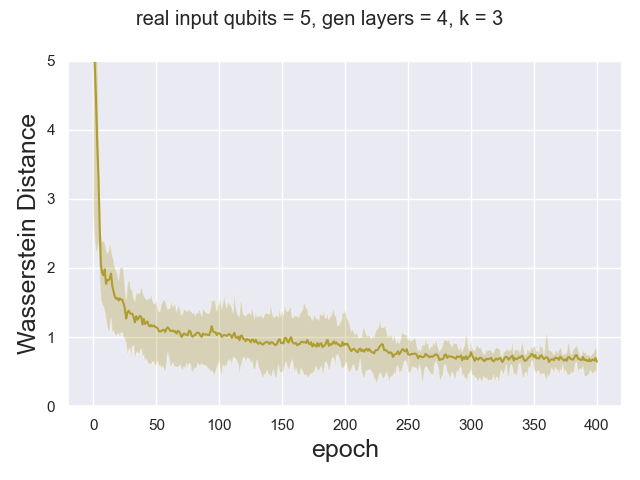
\includegraphics[width=0.25\linewidth]{figures/wqgans_butterfly_size=5_k=3_gen=4/Wasserstein_Distance.png}
  }
  \subfloat{
    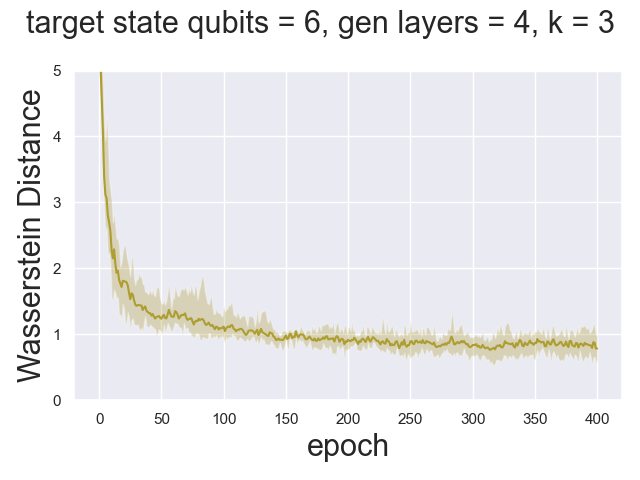
\includegraphics[width=0.25\linewidth]{figures/wqgans_butterfly_size=6_k=3_gen=4/Wasserstein_Distance.png}
  }
  \subfloat{
    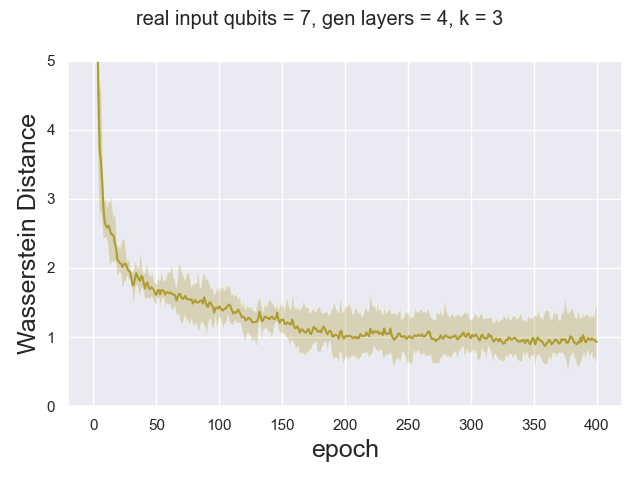
\includegraphics[width=0.25\linewidth]{figures/wqgans_butterfly_size=7_k=3_gen=4/Wasserstein_Distance.png}
  }
  \caption{Results of butterfly circuit estimation (ansatz Appendix \ref{apx:butterfly_ansatz}).
    The solid line represents the average value and the shaded area
    represents the range from 5 different experiments. The upper row shows the
    fidelity and the bottom row shows the corresponding Wasserstein distance. In all the
    experiments the generator is built using ansatz from \ref{apx:sqgans_ansatz}.}
  \label{fig:wqgans_res_butterfly_2}
\end{figure}
\begin{figure}[htbp!]
  \captionsetup[subfigure]{labelformat=empty}
  \centering
  \subfloat{
    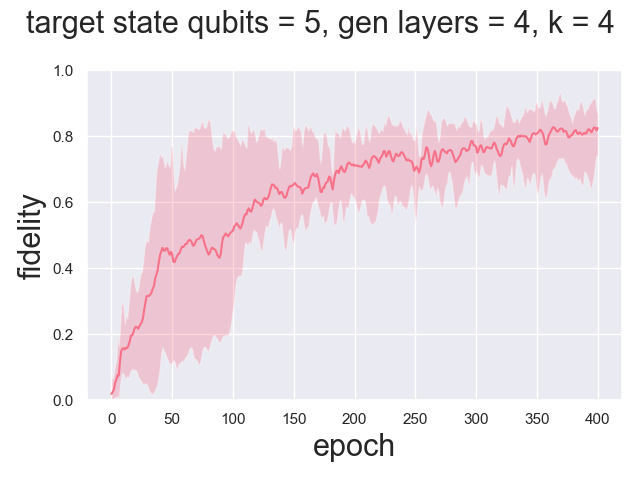
\includegraphics[width=0.25\linewidth]{figures/wqgans_butterfly_size=5_k=4_gen=4/fidelity.png}
  }
  \subfloat{
    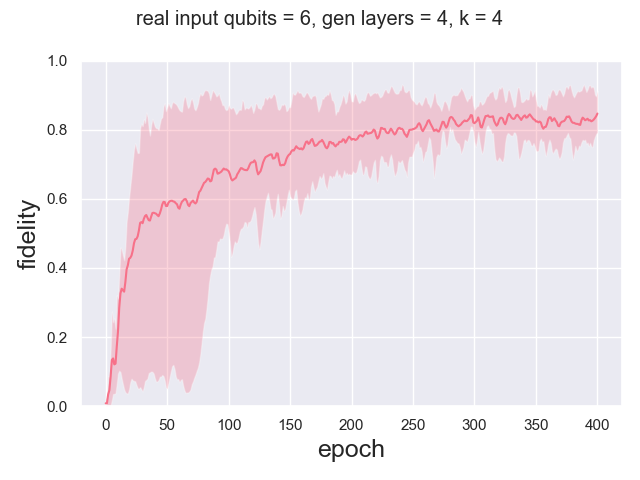
\includegraphics[width=0.25\linewidth]{figures/wqgans_butterfly_size=6_k=4_gen=4/fidelity.png}
  }
  \subfloat{
    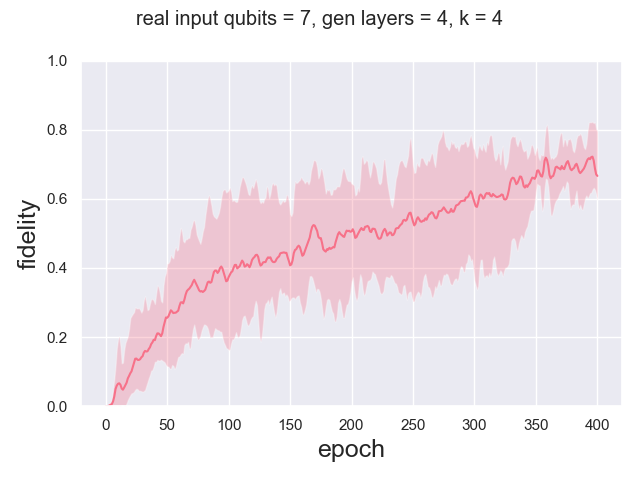
\includegraphics[width=0.25\linewidth]{figures/wqgans_butterfly_size=7_k=4_gen=4/fidelity.png}
  }
  \subfloat{
    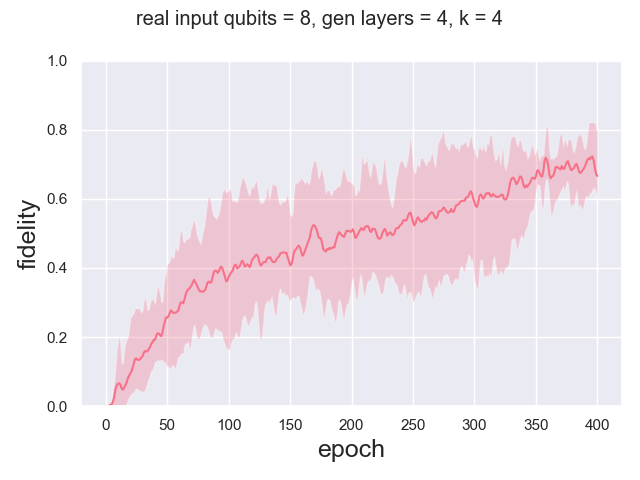
\includegraphics[width=0.25\linewidth]{figures/wqgans_butterfly_size=8_k=4_gen=4/fidelity.png}
  }

  \subfloat{
    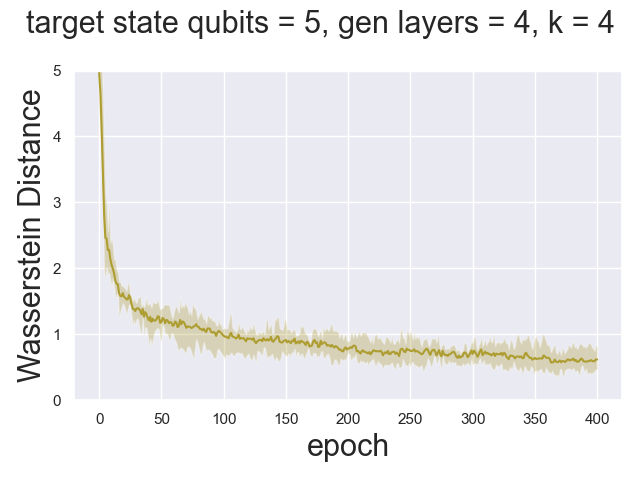
\includegraphics[width=0.25\linewidth]{figures/wqgans_butterfly_size=5_k=4_gen=4/Wasserstein_Distance.png}
  }
  \subfloat{
    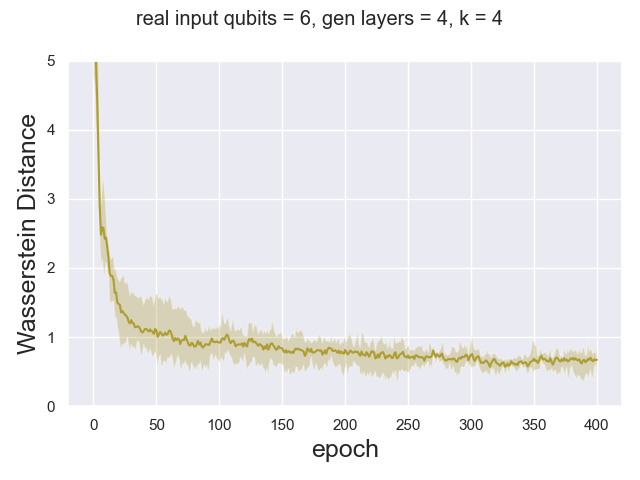
\includegraphics[width=0.25\linewidth]{figures/wqgans_butterfly_size=6_k=4_gen=4/Wasserstein_Distance.png}
  }
  \subfloat{
    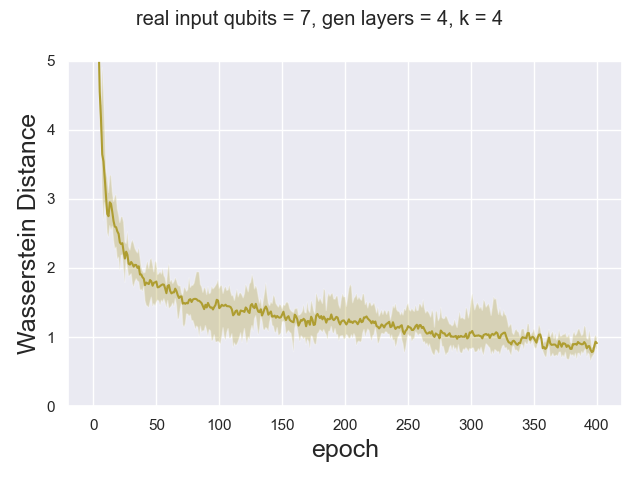
\includegraphics[width=0.25\linewidth]{figures/wqgans_butterfly_size=7_k=4_gen=4/Wasserstein_Distance.png}
  }
  \subfloat{
    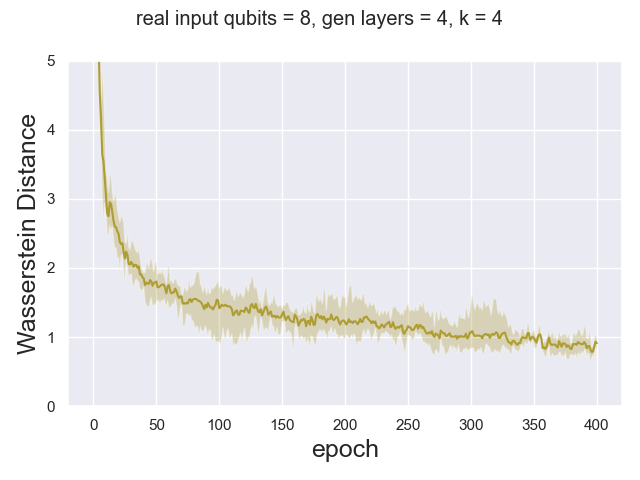
\includegraphics[width=0.25\linewidth]{figures/wqgans_butterfly_size=8_k=4_gen=4/Wasserstein_Distance.png}
  }
  \caption{Results of butterfly circuit estimation (ansatz Appendix \ref{apx:butterfly_ansatz}).
    The solid line represents the average value and the shaded area
    represents the range from 5 different experiments. The upper row shows the
    fidelity and the bottom row shows the corresponding Wasserstein distance. In all the
    experiments the generator is built using ansatz from \ref{apx:sqgans_ansatz}.}
  \label{fig:wqgans_res_butterfly_3}
\end{figure}
\let\clearpage\oldclearpage
% \section{Example 1}
% \cmark
% \section{Example 2}
% \xmark